\chapter{\albatros~Experiment}
\section{Overview of the Pathfinder}

\albatros~\citep[\albatros;][]{2020arXiv200812208C} pathfinder shown in Figure~\ref{Fig:albatros2} was introduced as an explorer in April 2018 at the \prizm\ site. Installing a pathfinder was a convenient way to assess Marion Island from discovering what is observable in the sky and finding out the observable frequencies. Figure~\ref{Fig:albatros2_schem} shows the block diagram of the pathfinder, and the signal chain description is below. The final experiment (\albatros) is aimed at consisting of autonomous antenna stations operating at a frequency range of \SIrange{1.2}{125}{\mega\hertz} that will map the low-frequency sky. Since these experiments are exploratory, they are taking steps towards achieving the future objective of coordinating observations to image the sky at frequencies that have been unexplored since the 1970s. These observations may allow us to probe even earlier epochs of the universe's history and will lay the groundwork for eventually exploring the cosmic "dark ages."

\begin{figure}
	\centering
	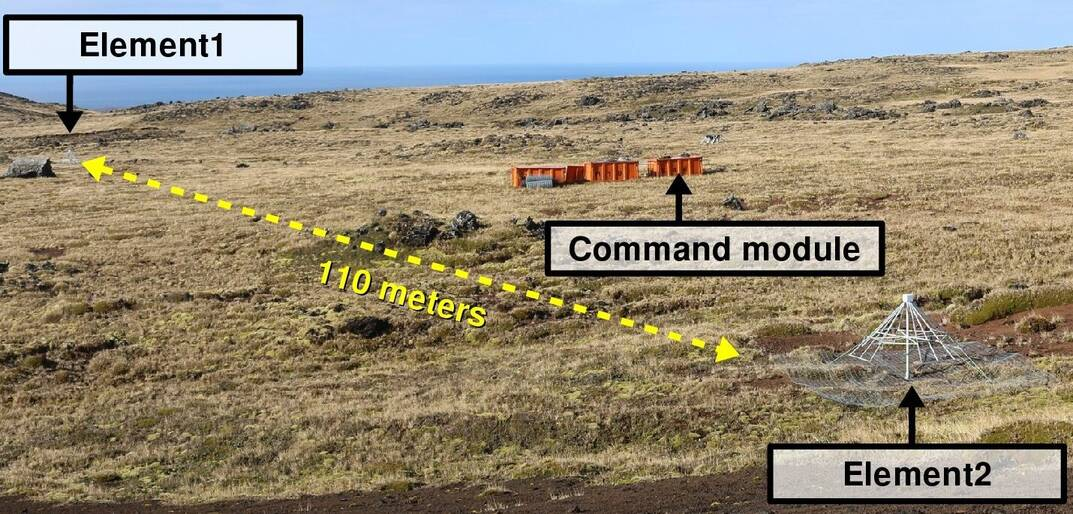
\includegraphics[width=\linewidth]{Figures/Albatros}
	\caption{The two-element, directly correlated \albatros\ pathfinder installed at the \prizm\ site. The pathfinder comprises two dual-polarization antennas separated by roughly 110 m on an east-west baseline. Coaxial cables connect the antennas to an orange shipping container that houses the readout electronics and serves as the "command module".}
	\label{Fig:albatros2}
\end{figure}

\section{Pathfinder System Signal Chain}

\begin{figure}
	\begin{center} 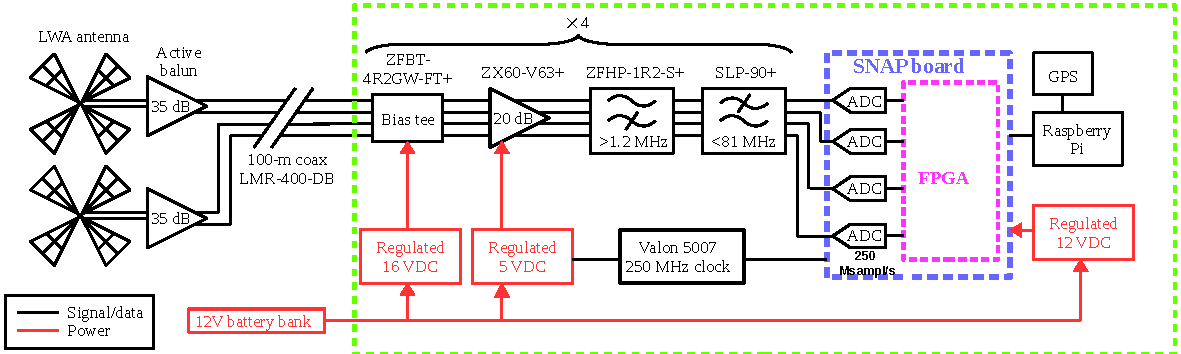
\includegraphics[width=\linewidth]{Figures/pathfinder_schematic.pdf}
		\caption{Two-element \albatros\ pathfinder block diagram.  Signals from two dual-polarzation LWA antennas are amplified by
			front-end active baluns~\citep{2012PASP..124.1090H}. The antennas are connected via 100-m coaxial cables to the back-end readout electronics, which are housed in a Faraday cage denoted by the green dashed box.  Each of the four antenna outputs is passed to a second-stage electronics chain consisting of filters and	further amplfication.  The signals are digitized at 250~Msamp/s by a SNAP board, which includes an on-board FPGA that computes auto- and cross-spectra from and between the four inputs.  A Raspberry Pi controls the SNAP board and saves the data.}
		\label{Fig:albatros2_schem}
	\end{center}
\end{figure}

\subsection{Antenna}\label{s:antenna}

The pathfinder uses two Long Wavelength Array (LWA) antennas configured as a two-element interferometric array. The two dual-polarization antennas are separated by $\sim$\SI{110}{\meter} on an east-west baseline. The dipole like antennas is of high preference for this project because they are relatively simple, and they are omnidirectionally patterned. The antennas possess low gain; therefore, the Galactic noise is limited by a fraction of 10, and the unwanted harmonics and intermodulation products are prevented~\citep{Memo28, Memo27}. The entire antenna and supporting structure sits on top of a ground screen that is roughly \SI{3}{\meter} on a side and is made of welded wire mesh.

\subsection{Front-end Electronics}\label{s:fee}

All the front end electronic (FEE) components are incorporated into a double-sided printed circuit board (PCB) as shown in Figure~\ref{Fig:balun} and the block diagram is shown in Figure~\ref{Fig:Balun Schematic}. One side of the PCB is populated with components, and the other side is a solid copper ground plane aperiodically stitched to the grounded copper on the side populated with components. The active balun provides an input impedance of \SI{50}{\ohm} to each dipole. The Mini-Circuits GALI-74+ monolithic microwave integrated circuit (MMIC) amplifiers from both feed points amplify each signal by +24 dB of gain. A passive {180\degree} hybrid coupler differentiates the two GALI-74+ outputs. A low-pass filters the coupler output by \SI{150}{\mega\hertz} and gains \SI{12}{\decibel} from the Mini-Circuits GALI-6+ MMIC. The signal gets fed to a second amplifier, and the output impedance of the FEE is matched to a \SI{50}{\ohm} \SI{100}{\meter} LMR400 coaxial cable having a nominal attenuation of $\sim$\SIrange{0.4}{3.7}{\decibel/100-m} at \SIrange{1.2}{81}{\mega\hertz}. The Mini-Circuits ZFBT-4R2GW-FT+ bias tee powers the FEE by \SI{16}{\volt} and extracts the RF signal by the use of the coaxial cable. The FEE has an overall gain of $\sim$ 36 dB and an overall noise figure of $\sim$ 2.7 dB to $\sim$ 2.9 dB~\citep{Memo35, 2012PASP..124.1090H}.

\begin{figure}
	\centering
	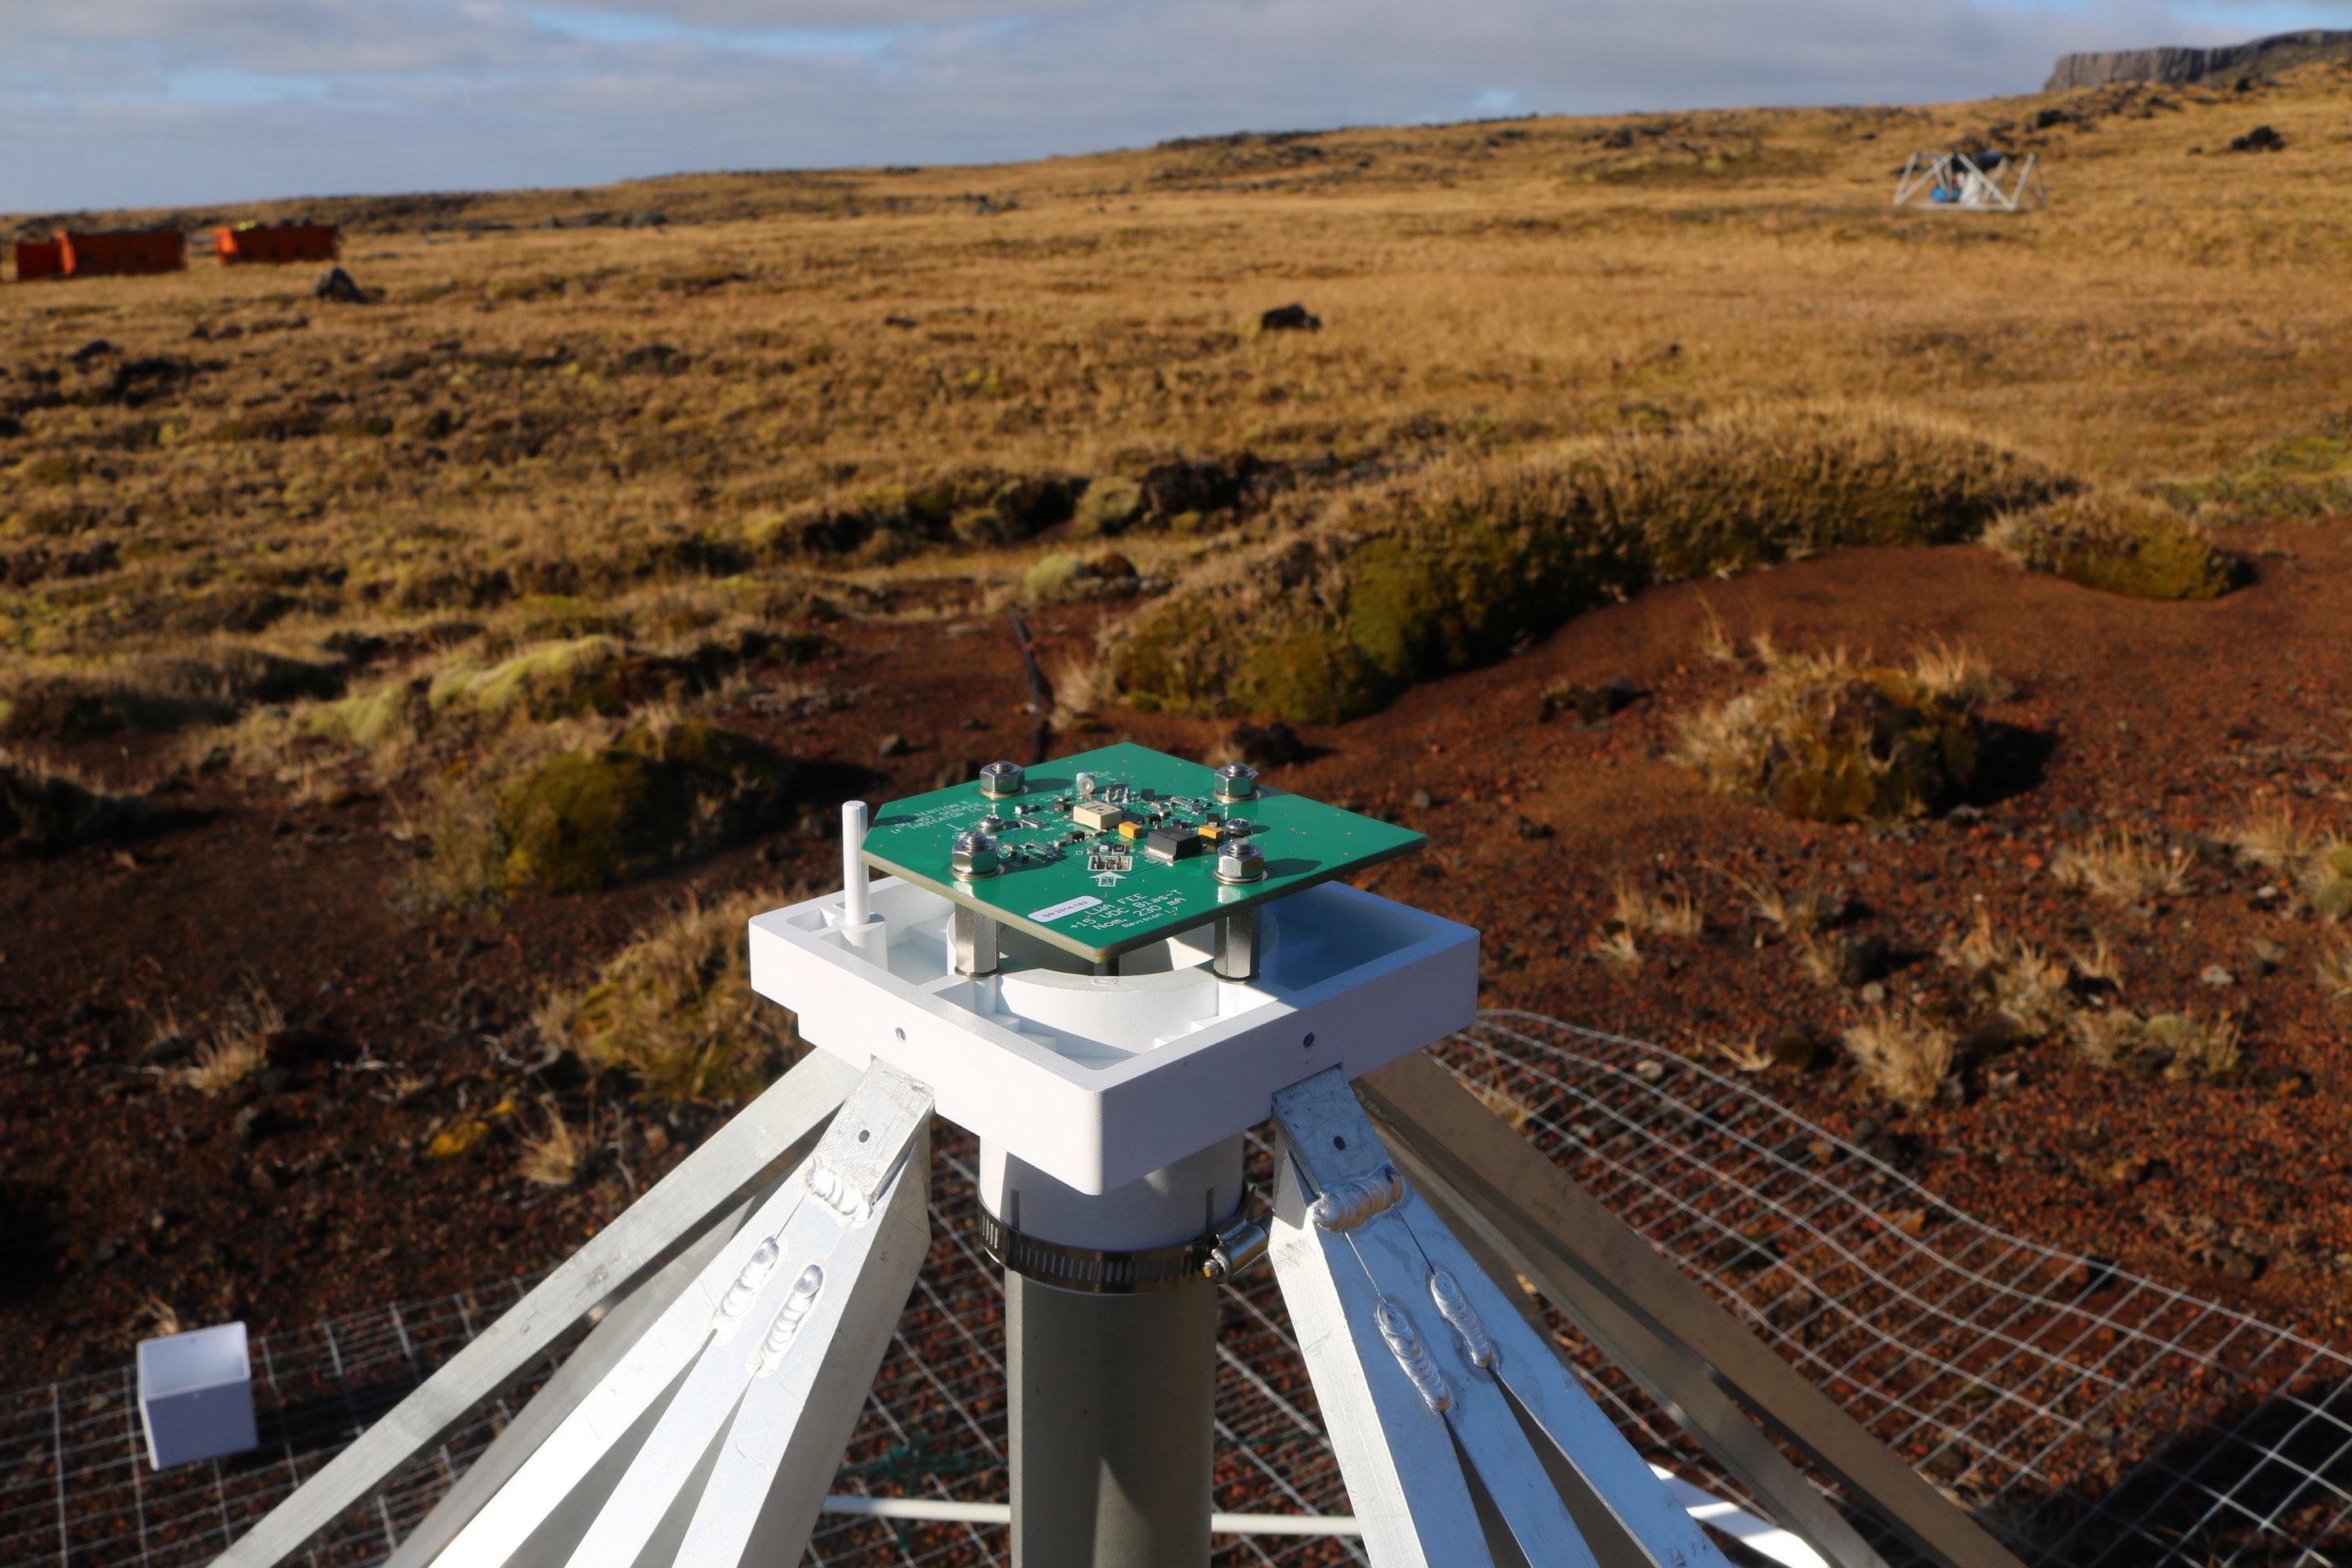
\includegraphics[width=\linewidth]{Figures/balun}
	\caption{Unenclosed FEE mounted on the pathfinder antenna supporting structure with the electronic components visible on the top part of the PCB.}
	\label{Fig:balun}
\end{figure}

\begin{figure}
	\begin{center}
		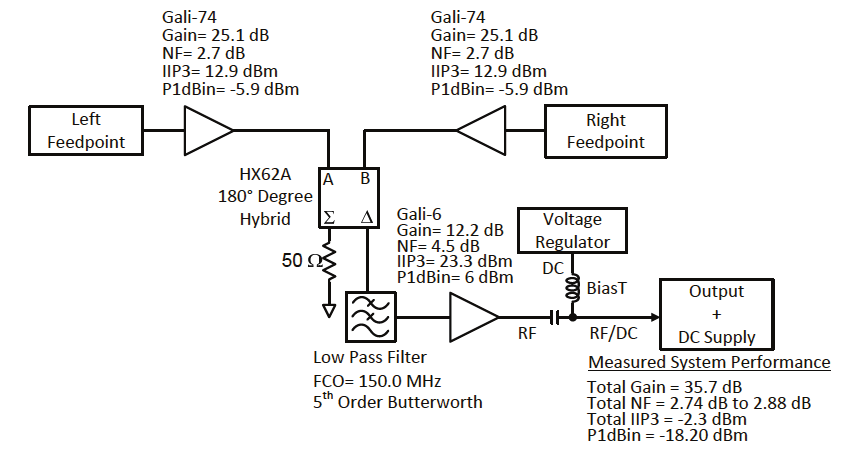
\includegraphics[width=\linewidth]{Figures/Balun_Block.png}
		\caption{One Polarisation Block Diagram of the FEE \cite{2012PASP..124.1090H}}
		\label{Fig:Balun Schematic}
	\end{center}
\end{figure}

\subsection{Back-end Electronics}

The back-end electronics are housed in the Faraday cage shown in Figure~\ref{fig:47093126504_fa0061a85b_o} denoted by the green dotted line box in Figure~\ref{Fig:albatros2_schem}. The analog signal chain consists of a Mini-Circuits ZX60-V63+ amplifier with a \SI{20}{\decibel} gain, and a pair of high- and low-pass filters (Mini-Circuits ZFHP-1R2+ and SLP-90+) that together band-limits the signal to \SIrange{1.2}{81}{\mega\hertz}. The amplifier operates at a frequency range of \SI{50}{\mega\hertz} - \SI{6}{\giga\hertz} and has a noise figure of $\sim$ 3.6 dB at its lowest operating frequency of \SI{\sim 50}{MHz}. The high- and low-pass filters present a nominal insertion loss of 0.2 dB and 0.14 dB at the center frequency of \SI{\sim10}{MHz}, respectively. 

\begin{figure}
	\centering
	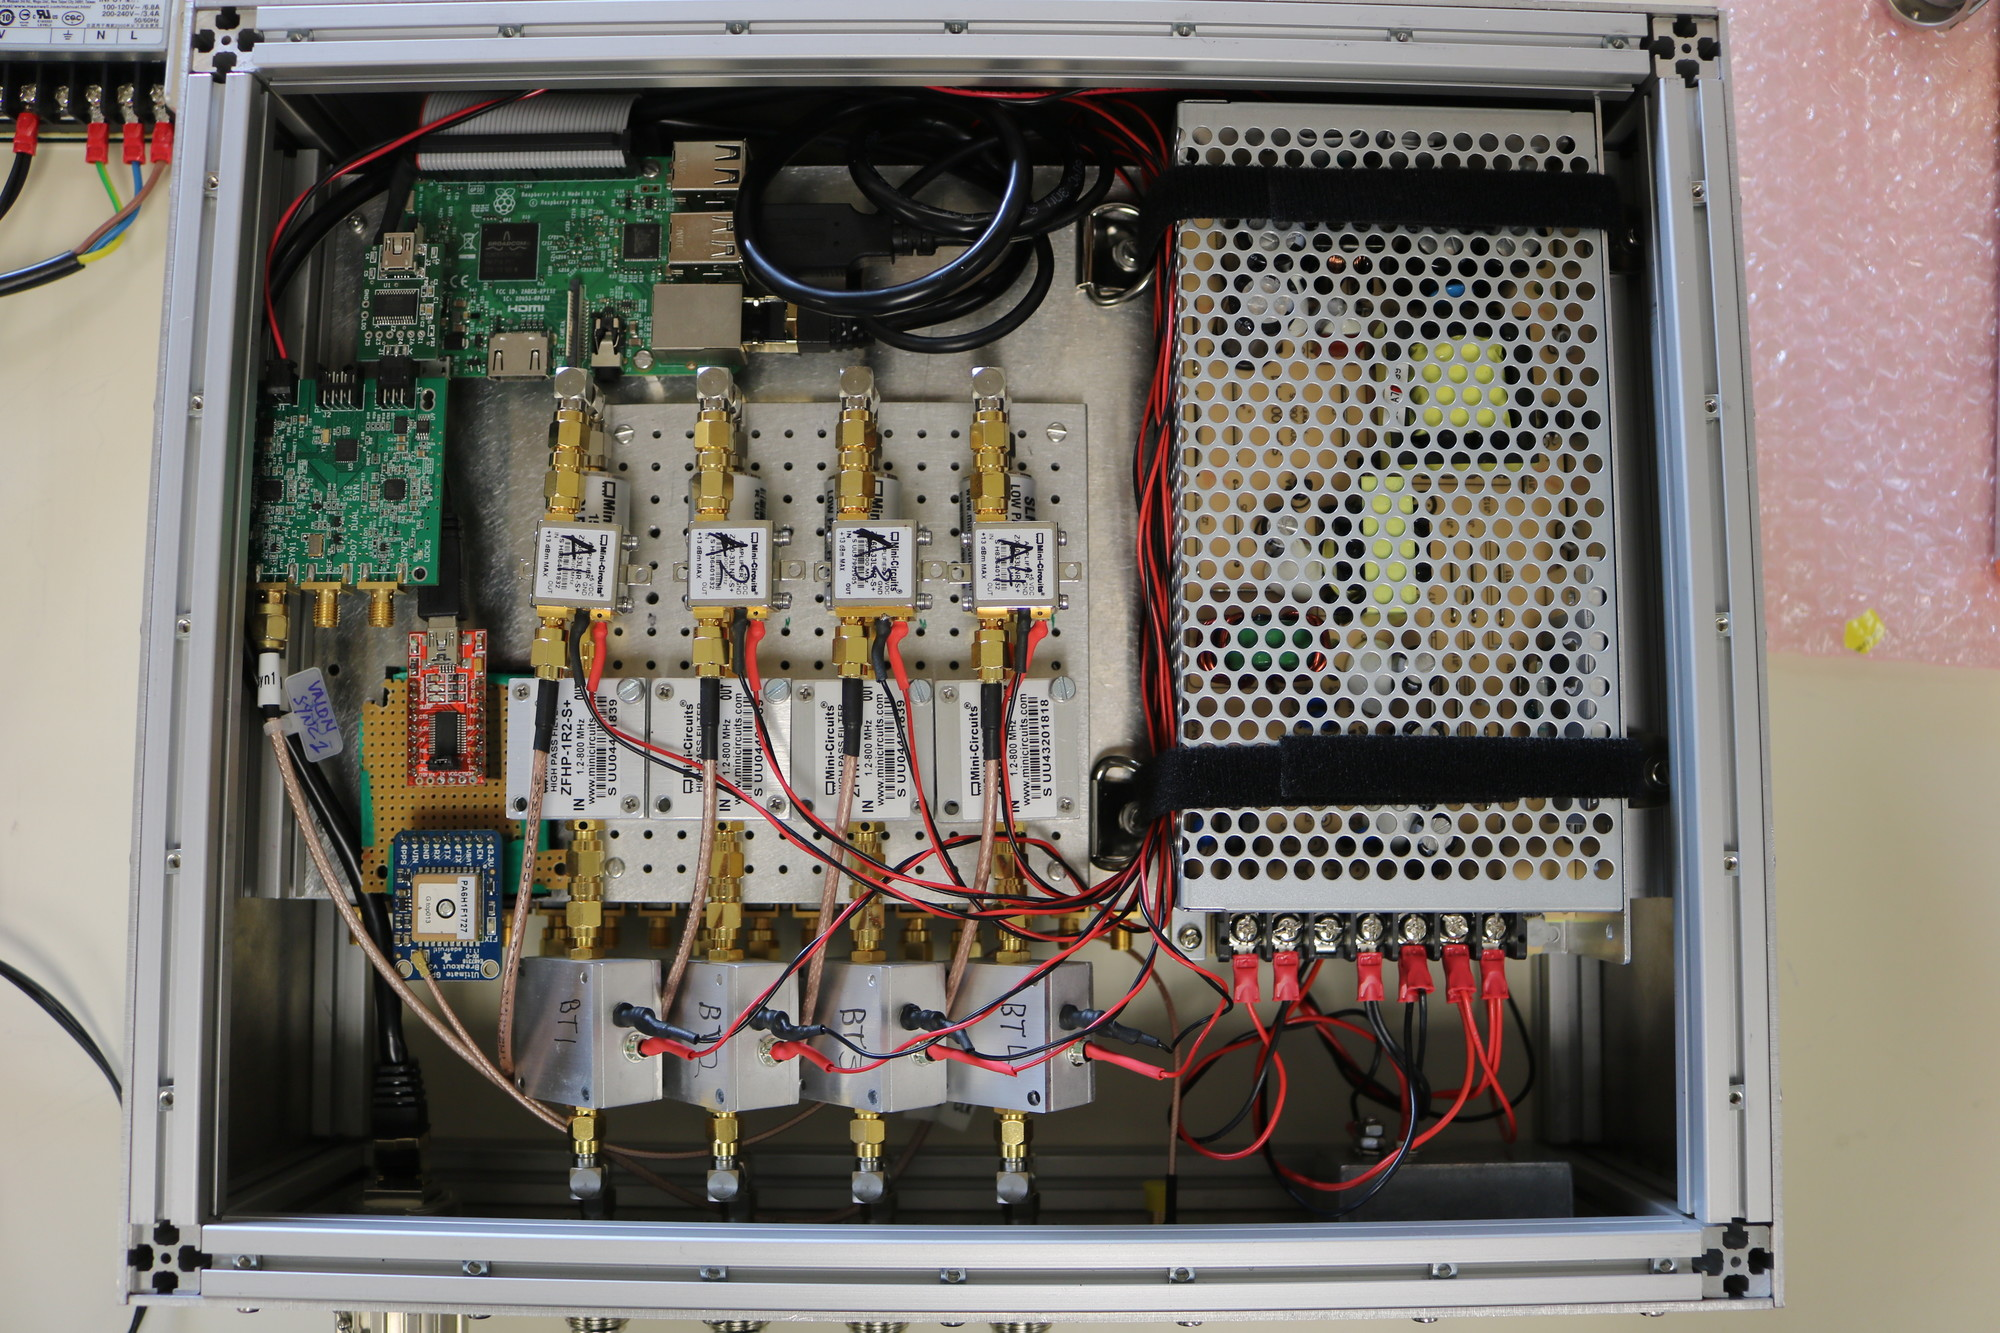
\includegraphics[width=\linewidth]{Figures/47093126504_fa0061a85b_o}
	\caption{\albatros\ back-end electronics housed in the Faraday cage. One side of the mounting plate shows the amplifiers, pair of high- and low-pass filters, bias-tees, Valon 5007 frequency synthesizer module, RPi and Adafruit Ultimate GPS module. Component not visible on this side are mounted on the other side of the mounting plate.}
	\label{fig:47093126504_fa0061a85b_o}
\end{figure}

A Smart Network ADC Processor~\citep[SNAP;][]{2016JAI.....541001H} mounted in the Faraday cage in Figure~\ref{fig:47093128324_04792aa5c5_o} samples the signals it receives by \SI{250}{Msampl/s} using an internal analog to digital converters (ADCs), and the signals of the clock are from the Valon 5007 frequency synthesizer module. A frequency range between \SIrange{0}{125}{\mega\hertz} containing 2048 channels is created by the SNAP board, which also includes the onboard Xilinx Kintex~7\footnote{\url{http://www.xilinx.com/products/silicon-devices/fpga/kintex-7.html}} FPGA that computes auto and cross spectra from and between the four inputs. A Raspberry Pi (RPi) controls the SNAP board and saves data to an onboard SD-card. The RPi absolute timing is provided by Adafruit Ultimate GPS module\footnote{\url{https://www.adafruit.com/product/746}}, connected
to an active external GPS antenna.

\begin{figure}
	\centering
	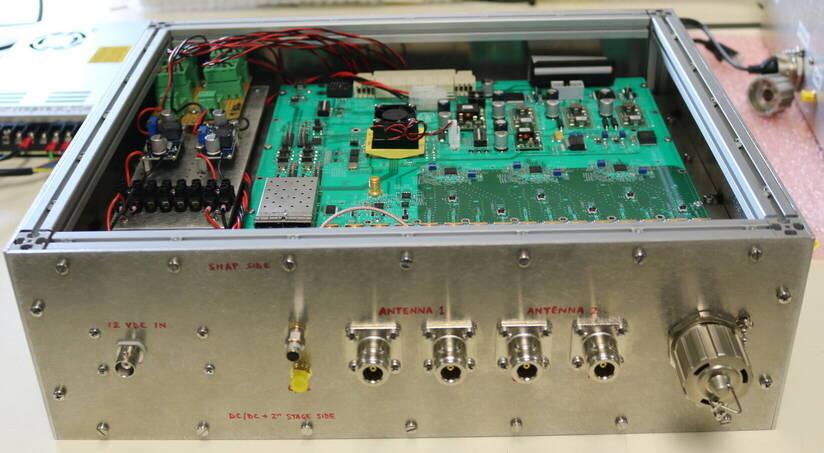
\includegraphics[width=0.8\linewidth]{Figures/47093128324_04792aa5c5_o}
	\caption{The bottom side of the \albatros\ Faraday cage, showing the mounted SNAP board and the regulatory circuit. }
	\label{fig:47093128324_04792aa5c5_o}
\end{figure}

\subsection{Power}
The two-element pathfinder system is powered using four \SI{12}{\volt} \SI{200}{\ampere\hour} battery bank wired in parallel and battery charging is performed manually using a Honda EU30is\footnote {\url{http://www.hondaenergy.com/generators/honda-eu30is.html}} generator and a fuel cache that is kept at the observing site. The main advantage and encouragement to use a SNAP board is its low power consumption, which is feasible for the power supply method. The total system power draw is \SI{\sim45}{\watt} and the pathfinder system can operate without interruption for $\sim$1 week when the batteries are fully charged. During observations, the batteries are connected to DC/DC converters powering the SNAP board, FEE, amplifiers, and the clock. The DC-DC converters are housed inside the Faraday cage and provide stable voltage outputs	despite the slow decline of the battery voltage.

\section{Overview of Autonomous Stations}

The final ALBATROS array will consist of ten autonomous antenna stations (huts) separated by baselines of \SI{\sim {20}}{km} as shown in \autoref{Fig:marion_map}. Marion Island huts, which are potential stations for the ALBATROS array, have a ring-like pattern which is appropriate for imaging and produces an FWHM synthesized beam of $7'$ at \SI{5}{\mega\hertz} as shown in \ref{fig:marion_map_beam}. The array beam promises an improved resolution over existing measurements to date. Thus far, the ALBATROS main goal will be to map high resolutions at low frequencies, which is crucial before doing cosmological observations of the dark ages. 

In April 2019, I was part of the deployment team in Marion Island, and I am going to discuss in detail the tasks associated with \albatros\ that we managed to complete during the three weeks relief voyage.  

\begin{figure}
	\centering
	\begin{subfigure}[t]{0.6\textwidth}
		\centering
		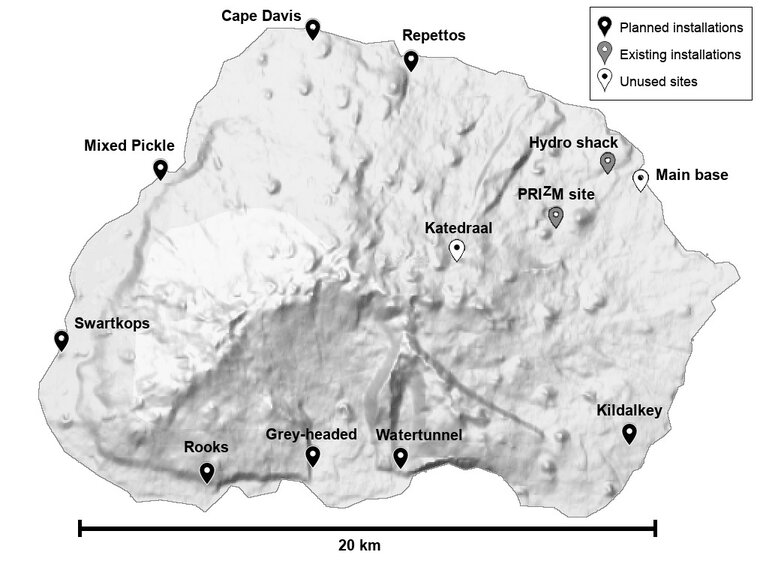
\includegraphics[width=\linewidth]{Figures/marion_map_annotated.jpg} 
		\caption{} \label{Fig:marion_map}
	\end{subfigure}
	\hfill
	\begin{subfigure}[t]{0.39\textwidth}
		\centering
		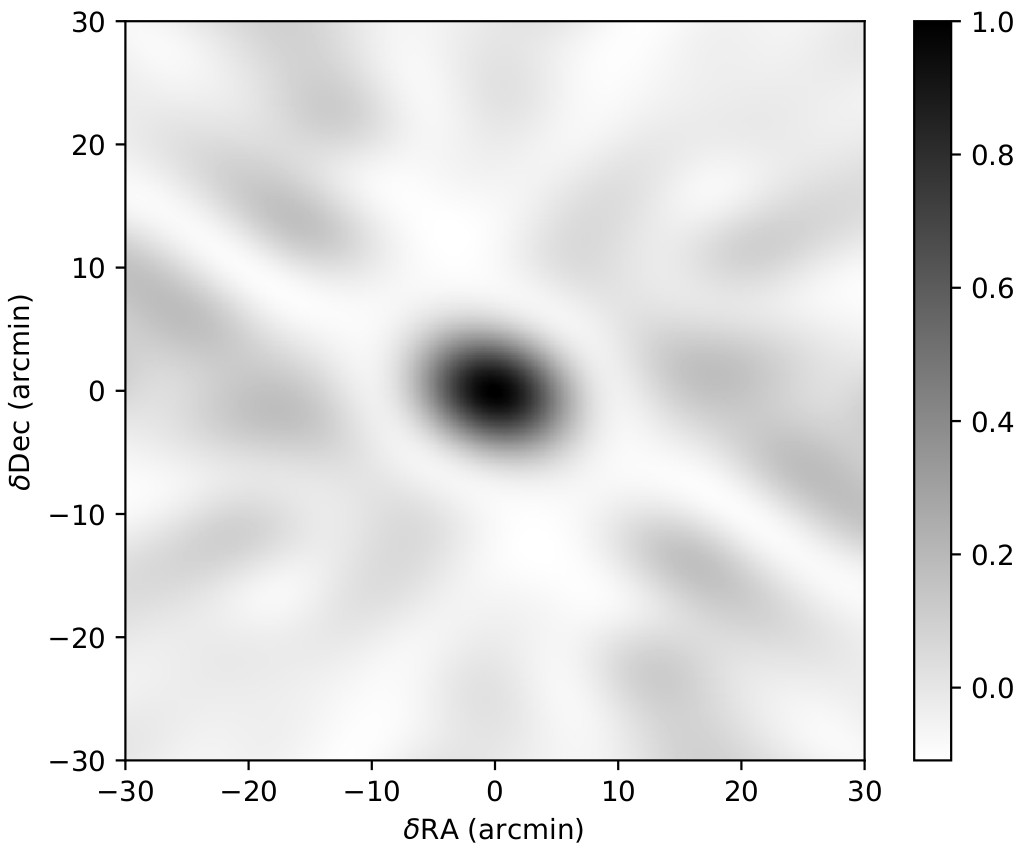
\includegraphics[width=\linewidth]{Figures/marion_beam_huts_2020.jpg}
		\caption{} \label{Fig:marion_beam}
	\end{subfigure}
	\caption{{\bf (a)} Map of Marion Island.  The
		\albatros\ pathfinder antennas are currently installed at the
		\prizm\ site and at the hydro shack (gray markers).  The black
		markers denote the eight coastal huts, which will be used for
		future \albatros\ antenna installations.  The white markers
		denote other available infrastructure points that will not be
		used for antennas. {\bf (b)} Synthesized beam at 5~MHz at zenith from the full \albatros\ array, using the existing and planned
		installation locations shown on the map.  Using an octave of
		bandwidth spanning 3.5--7~MHz in a single snapshot, we obtain a synthesized beam with a full width of $\sim7'$.}\label{Fig:marion_map_beam}
\end{figure}

\section{2019 Marion Voyage}

The S. A. Agulhas II sails from Cape Town each year in April. The relief voyage preparations begin months before the ship sails; the team plans and makes decisions based on the next voyage's goals. The development and testing of improved designs and systems occur at the University of KwaZulu Natal radio astronomy lab. In preparation for the 2019 voyage, I designed and developed a prototype solar power supply system that paved the way for the solar power supply system installed in Marion Island as part of the autonomous stations. Because of the weather conditions in Marion Island, the pathfinder system can shut down for an extended period without observations. Thus, a solar power system solution was implemented on the first autonomous station to run the system autonomously continuously. 

During the relief voyage, the installation process included mechanical assembly and alignment of the antenna structure itself, laying coaxial cables, installing three solar panel mounts (with three panels each, for a total of nine panels), and installing a small processing hub consisting of a plastic bin housing the readout electronics, two batteries, and power control electronics. The first autonomous station signal chain shown in Figure~\ref{Fig:albatros1_schem} was installed in April 2019 at the hydroshack site (\ang{46;52.205;}S, \ang{37;50.612;}E) on Marion Island as a first step in testing the technology needed to create the full array. A similar antenna and front end active balun discussed in (\S\ref{s:antenna} and \S\ref{s:fee}) were used, and the back-end electronics and the power system are discussed in detail below.

\section{Autonomous Stations Signal Chain}

\begin{figure}
	\begin{center}
		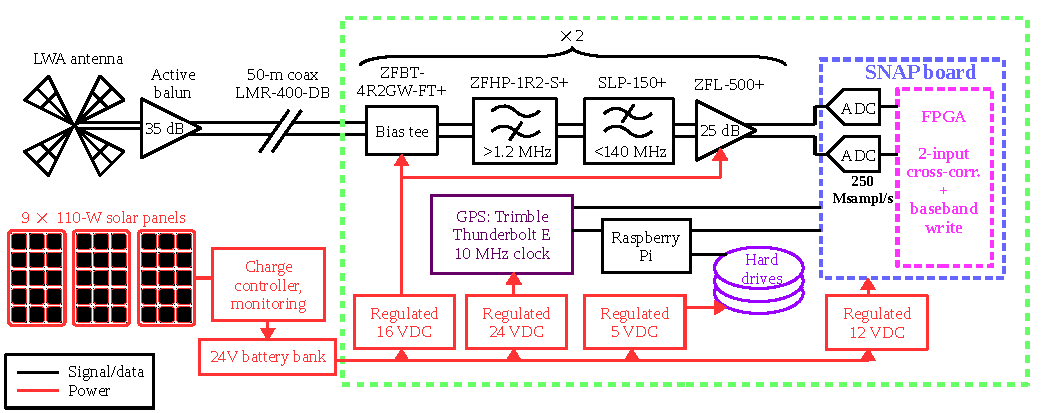
\includegraphics[width=\linewidth]{Figures/albatros_single_schematic.pdf}
		\caption{Single-antenna autonomous station block diagram. A dual-polarization LWA antenna, equipped with an active front-end balun, connects via 50-m coaxial cables to the back-end readout electronics, housed in a Faraday cage denoted by the green dashed box. Each of the two antenna signals is passed to a second-stage electronics chain consisting of filters and further amplification.  The signals are digitized at 250~Msamp/s by a SNAP board, including an onboard FPGA that computes channelized baseband and spectra from both inputs.  A Raspberry Pi controls the SNAP board and receives the baseband data and spectra.  The baseband data are saved to external hard drives. The system is powered by solar panels that charge a 24-V battery bank.}
		\label{Fig:albatros1_schem}
	\end{center}
\end{figure}

\subsection{Back-end Electronics} 

\begin{figure}
	\centering
	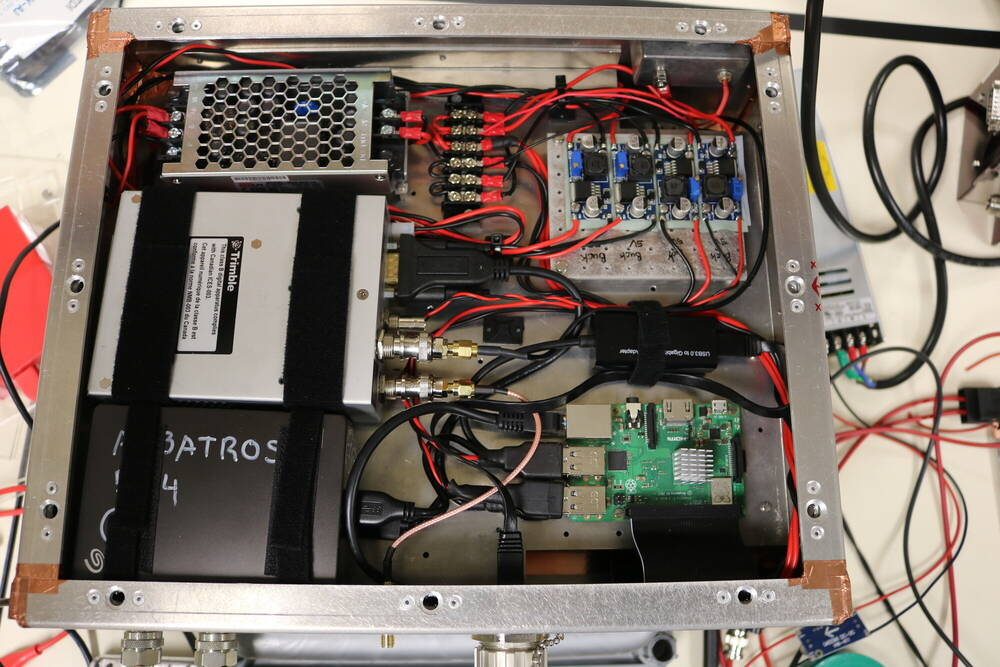
\includegraphics[width=0.7\linewidth]{Figures/46966493985_44aa8ac326_o}
	\caption{The single autonomous station Faraday cage showing one side of the mounting plate with visible power distribution circuitry, Trimble Thunderbolt E GPS-disciplined clock module, external hard drives and the RPi.}
	\label{fig:46966493985_44aa8ac326_o}
\end{figure}

The Faraday cage shown in Figure~\ref{fig:46966493985_44aa8ac326_o} denoted by the green dotted line box in Figure~\ref{Fig:albatros1_schem} is located \SI{50}{\meter} away from the antennas. The analog signal chain shown in Figure~\ref{fig:47882594521_3895effd86_o} on the other side of the mounting plate in the RF partition consists of a pair of high- and low-pass filters (Mini-Circuits ZFHP-1R2+ and SLP-150+) that together band-limit the signal to \SIrange{1.2}{140}{\mega\hertz}, and after the filters is the Mini-Circuits ZFL-500+ amplifier with a \SI{25}{\decibel} typical gain. The amplifier operates at a frequency range of \SIrange{0.05}{500}{\mega\hertz}. Figure~\ref{fig:foo} shows a comparison between the amplifier used on the two-element pathfinder and the single autonomous station. The plot shows an improved gain response; the ZFL-500+ amplifier response is flatter and is well within the experiment's operating frequency.

\begin{figure}
	\begin{center}
		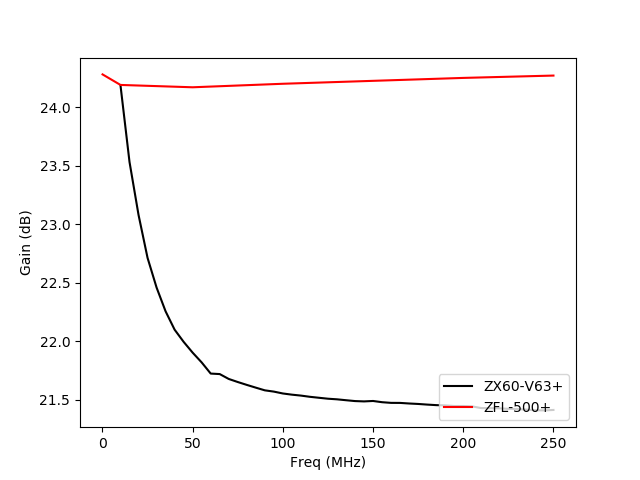
\includegraphics[width=0.8\linewidth]{Figures/foo.png}
		\caption{The comparison plot of S21 (gain) for the two-element pathfinder and the single autonomous station amplifier.}
		\label{Fig:foo}
	\end{center}
\end{figure}

\begin{figure}
	\centering
	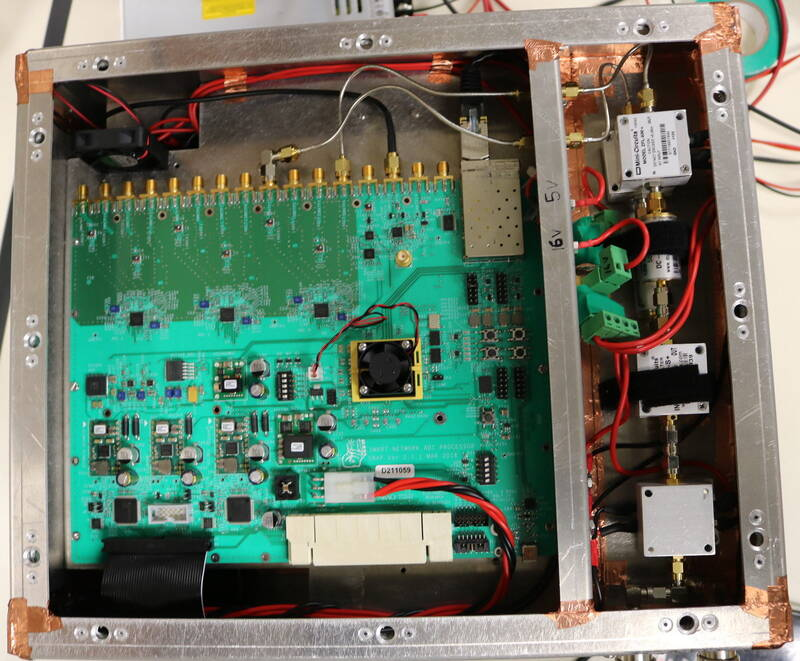
\includegraphics[width=\linewidth]{Figures/47882594521_3895effd86_o}
	\caption{The single autonomous station Faraday cage with the analog signal chain mounted in the RF partition on the left and the SNAP board mounted on the right.}
	\label{fig:47882594521_3895effd86_o}
\end{figure}


In comparison to the two-element pathfinder, the cut-off frequency of the low-pass filter increased from \SIrange{81}{140}{\mega\hertz} to capture downlink signals at \SIrange{137}{138}{\mega\hertz} from the ORBCOMM satellite constellation. The ORBCOMM signals are beneficial to the final \albatros\ array because they provide a convenient means for synchronization across the antenna stations, serving as a backup to the GPS timing discussed below. Actual lab tests recommend that on time scales of \SI{\sim 30}{\second}, relative timing between various autonomous stations can be estimated to a precision of better than a couple of tenths of a nanosecond utilizing a solitary satellite. At \SI{10}{\mega\hertz} the correlation phase error is $\lesssim1^\circ$. With open-access orbits and various satellites commonly within the field of view, the ORBCOMM baseband data supposedly saved simultaneously with the astronomical data can provide offline synchronization of the ALBATROS stations. Since the ORBCOMM and science data are recorded simultaneously by the same system, enhancement to the timing calibration can be applied in post-processing.

The signals are then digitized at \SI{250}{Msampl/s} by the SNAP board mounted in the Faraday cage in Figure~\ref{fig:47882594521_3895effd86_o}. A Trimble Thunderbolt E GPS-disciplined clock module creates a \SI{10}{\mega\hertz} reference that is locked from the SNAP board internal ADCs. The SNAP board FPGA processes channelized baseband data for every polarization over tunable frequency windows inside the \SIrange{0}{125}{\mega\hertz} range, with the options of 1-, 2-, 4-bit baseband channelization, and auto-and cross-spectra from the two polarizations over the full \SIrange{0}{125}{\mega\hertz} range, collected more than few-second spans. The decrease in bit profundity happens simply after the SNAP board has channelized the baseband, and the cross-channel spillage (due to, e.g., RFI and inclines in RF power as observed by the ADCs) is thusly unaffected by the low bit profundity. 

An RPi 3B+ controls the SNAP board and gets the auto-and cross-spectra through GPIO pin connections, and the spectra are saved to an onboard SD card. The baseband data is passed through an ethernet from the SNAP board to the RPi and saved to external hard drives. The presentation of gigabit ethernet with the RPi 3B+ model has empowered the high data throughput related to writing baseband. As a benchmark, 1-bit baseband recording of two polarizations more than \SI{10}{\mega\hertz} of transmission capacity yields an inexact data rate of 5~MB/s or 400~GB/day.

\subsection{Correlation}


\subsection{Solar Power Supply System}

The future autonomous stations shown in Figure~\ref{Fig:marion_map} are farther from the island's main base; hence, the development of autonomous power supply systems. A solar power supply system was developed for the first autonomous station installed at the hydroshack site. The system is powered using an array of nine SunPower SPE-E-Flex-110 solar panels that charge a \SI{24}{\volt} battery bank made up of two series-connected, 12 V, deep cycle, lead-acid batteries. Each solar panel has a nominal power of \SI{110}{\watt}, capable of producing an open circuit voltage of approximately \SI{22.8}{\volt} and \SI{6.3}{\ampere}. On account of the extremely incessant cloudy conditions on Marion Island, the charging capacity of \SI{1}{\kilo\watt} is deliberately immense for the required \SI{\sim 50}{\watt} to run the station.

\begin{figure}
	\centering
	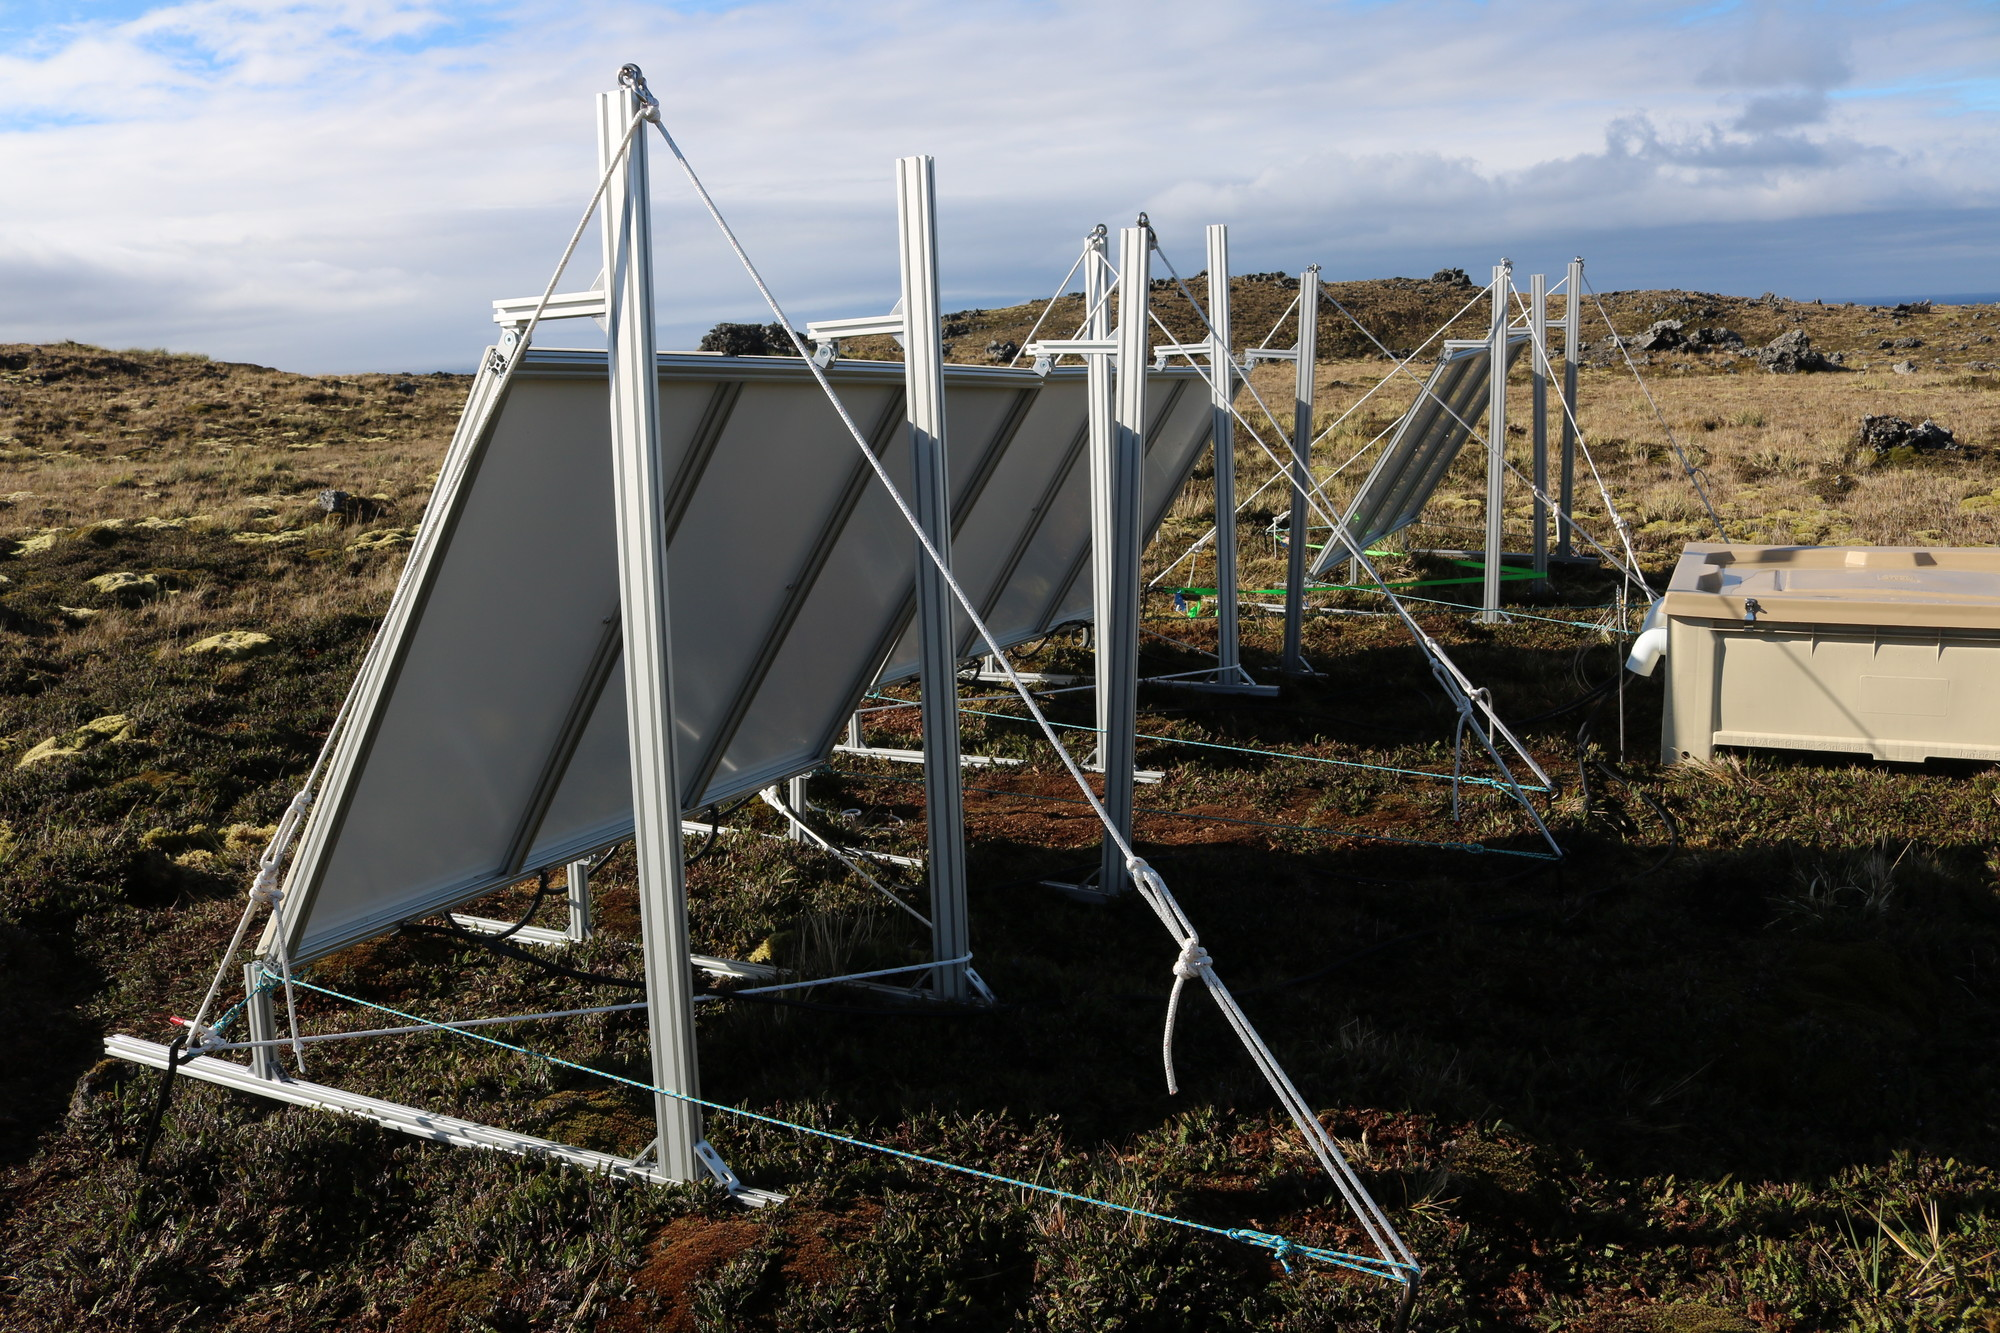
\includegraphics[width=\linewidth]{Figures/40916139043_f3d0c6b013_o}
	\caption{}
	\label{fig:40916139043_f3d0c6b013_o}
\end{figure}

The supporting structures for the nine solar panels were specifically designed to manage the gale-force winds on Marion Island, though it was challenging to install them as the volcanic ground minimizes the appropriate anchoring ability. The three aluminum mounting structures each carry three solar panels mounted on a rigid metalized plastic panel. The structures are oriented due north and are designed to incline the solar panels at a relatively steep angle to perform efficiently under winter conditions. The three supporting structures with mounted solar panels are shown in Figure~\ref{fig:40916139043_f3d0c6b013_o}. Behind the supporting structures is the plastic enclosure housing the readout electronics, two batteries, and the power control electronics shown in Figure~\ref{fig:bin}.

\begin{figure}
	\centering
	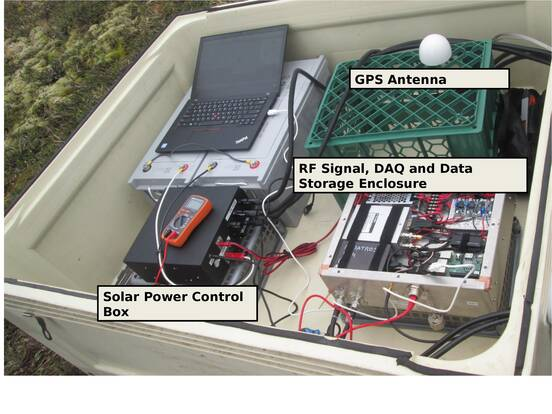
\includegraphics[width=0.7\linewidth]{Figures/bin}
	\caption{}
	\label{fig:bin}
\end{figure}


Each of the three solar panel sets is connected in series and parallel to the Victron BlueSolar MPPT 50|35 charge controller, optimizing power transfer from the solar array when charging is required, and monitors charge level reducing output current when the battery bank is fully charged. An Arduino logs the data from the Victron charge controller to an SD card and switches power on and off to the readout electronics box. The on/off feature is compulsory to avert battery system damage from excessively deep discharge. The system also has a battery power conservation feature, which schedules observations for distinct periods, often during the night when ionospheric conditions are more favorable. The power logging and control system, the Victron charge controller, and an EMI filter are housed together in an aluminum box shown in Figure~\ref{fig:power_box_interior}. The solar charge controller generates RF noise, which would likely cause interferences; hence, an EMI filter was designed to minimize conducted emissions on the solar charge controller's photovoltaic side. Figure~\ref{fig:station} shows the complete installation of the first autonomous station.

\begin{figure}
	\centering
	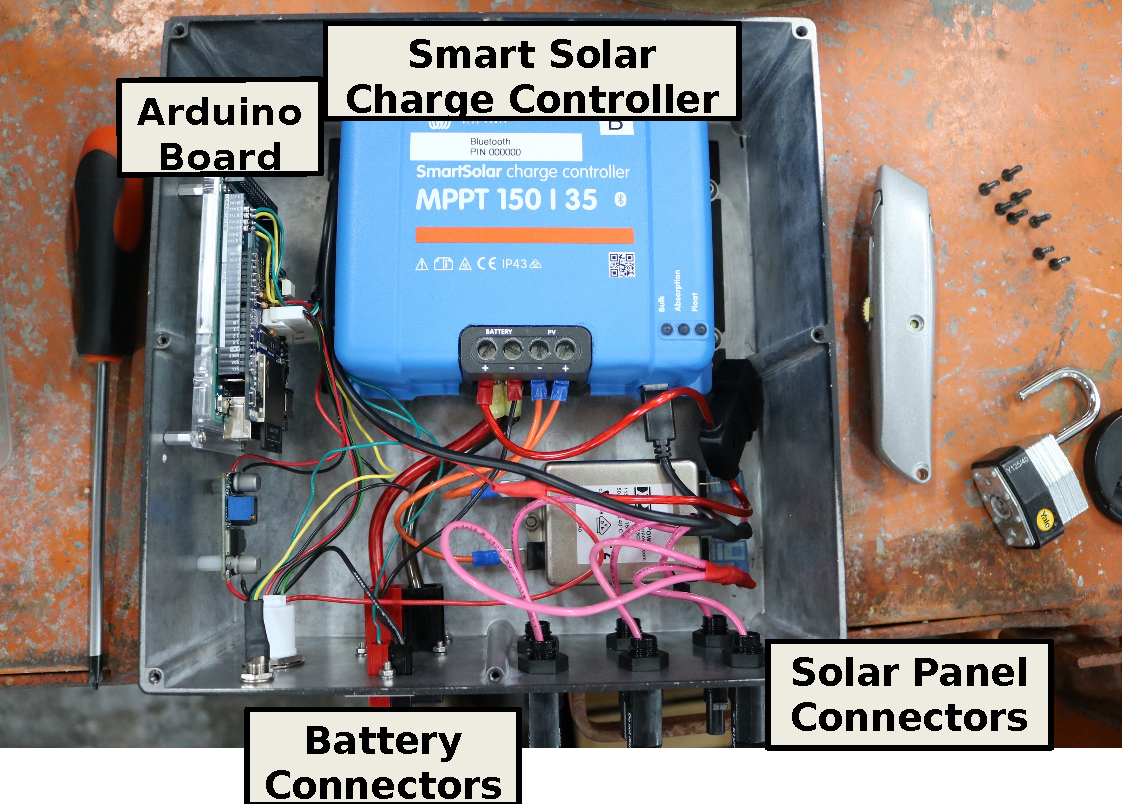
\includegraphics[width=\linewidth]{Figures/power_box_interior}
	\caption{}
	\label{fig:power_box_interior}
\end{figure}

\begin{figure}
	\centering
	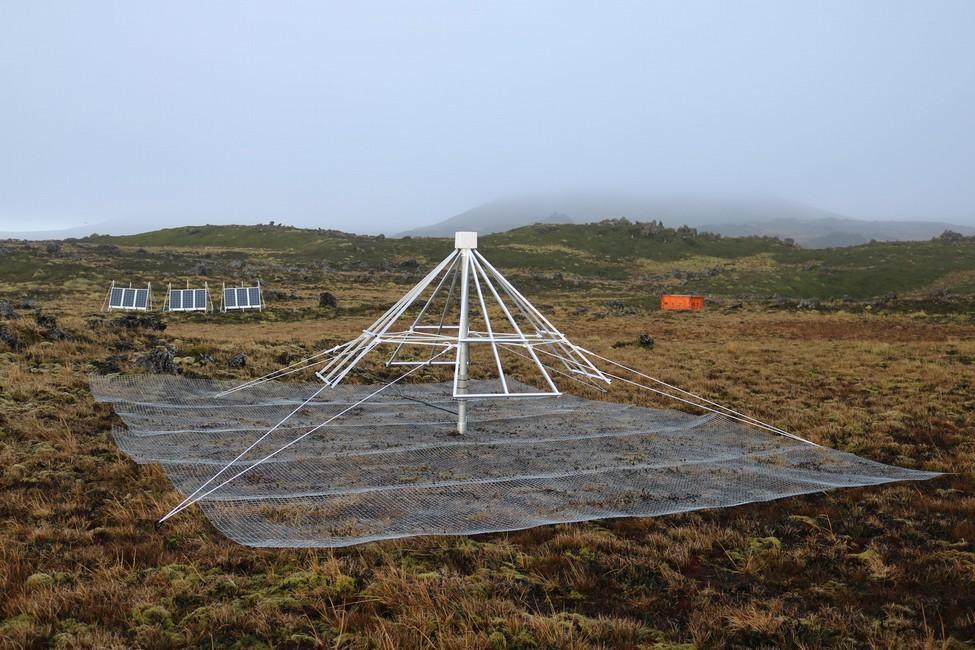
\includegraphics[width=\linewidth]{Figures/station}
	\caption{}
	\label{fig:station}
\end{figure}
